\chapter{Real-Life Drug Discovery Case Studies}

Our colleges and collaborators as biochemists and pharmacists are working on several high-impact drug discovery projects. They have done lots of biological assays and succeeded in identifying pharmaceutical and druggable protein targets for certain diseases. They outsource the docking tasks to us, hoping to discover potent and selective inhibitors of certain proteins.

\section{Influenza A Virus H1N1}

Prof. P.C. Shaw from Department of Biochemistry at Chinese University of Hong Kong and his team have studied influenza A virus H1N1 (swine flu) for years. They select the influenza viral nucleoprotein and the influenza A RNA polymerase subunit PA as drug targets, and we assist with structure-based virtual screening.

The influenza viral nucleoprotein forms the protein scaffold of the helical genomic ribonucleoprotein complexes, and interacts with the viral RNA polymerase to promote viral RNA replication. Oligomerization of the nucleoprotein is mediated by a flexible tail loop that is inserted into the body domain of a neighbouring molecule and makes extensive interactions through intermolecular $\beta$-sheets, hydrophobic interactions and salt bridges (Figure \ref{Case:InfluenzaNucleoprotein}, reprinted from \citep{1140}). The displacement of the tail loop from its binding pocket causes significant structural rearrangements in nucleoprotein. Chemical compounds which competitively displace the tail loop from its binding pocket would interfere with viral genome replication, and therefore serve as promising leads for anti-influenza drug development \citep{1140}.

\begin{figure}
\centering
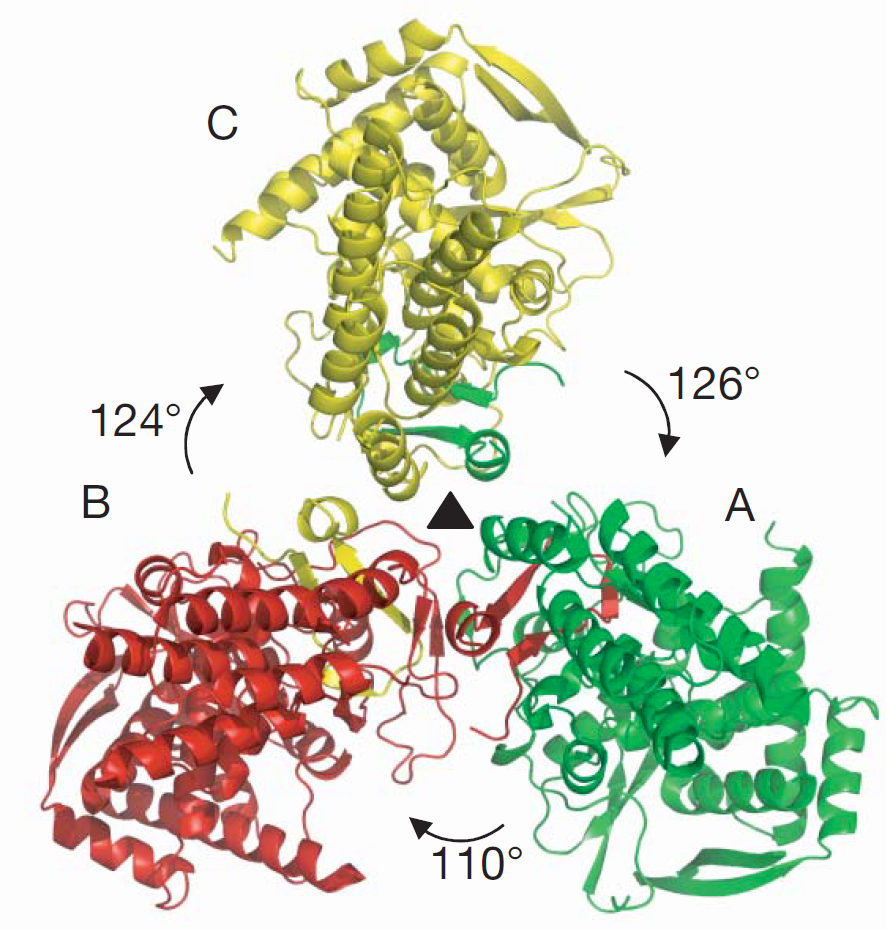
\includegraphics[width=\linewidth]{Case/InfluenzaNucleoprotein.png}
\caption{Nucleoprotein trimer viewed along the NCS (Non-Crystallographic Symmetry) three-fold axis, with three subunits shown in different colours. The rotation angles that relate the three subunits are marked. Figure reprinted from \citep{1140}.}
\label{Case:InfluenzaNucleoprotein}
\end{figure}

The three subunits of influenza A RNA polymerase, namely PA, PB1 and PB2, are required for both transcription and replication. PA is involved in assembly of the functional complex, cap binding and virion RNA (vRNA) promoter binding, while PB1 carries the polymerase active site. The carboxy-terminal domain of PA forms a novel fold, and forms a deep, highly hydrophobic groove into which the amino-terminal residues of PB1 can fit by forming a helix and interact through an array of hydrogen bonds and hydrophobic contacts (Figure \ref{Case:InfluenzaPAPB1}, reprinted from \citep{1141}). The loss of PA abolishes RNA polymerase activity and viral replication. PA and its interface with PB1 are therefore potential drug targets \citep{1141}.

\begin{figure}
\centering
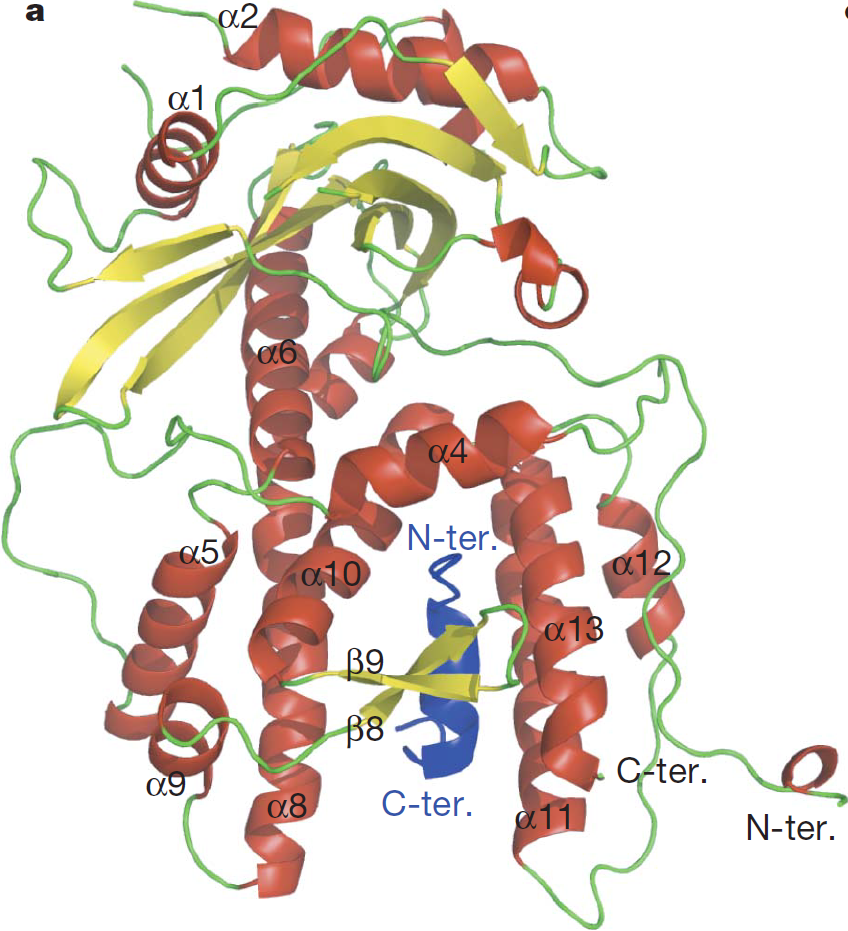
\includegraphics[width=\linewidth]{Case/InfluenzaPAPB1.png}
\caption{Crystal structure of the C-terminal domain of PA bound to the N-terminal peptide of PB1, coloured dark blue. Figure reprinted from \citep{1141}.}
\label{Case:InfluenzaPAPB1}
\end{figure}

We obtain the X-ray crystal structures of influenza viral nucleoprotein with PDB ID 2IQH and influenza A RNA polymerase subunits PA-PB1 complex with PDB ID 2ZNL. For the nucleoprotein, we remove protein chains B and C and only retain chain A. For the PA-PB1 complex, we remove PB1 and only retain PA. With idock 1.4, we start virtual screening 7,220,835 ZINC \citep{532} clean ligands whose molecular weight is above 350g/mol against the nucleoprotein chain A. The 7 million ligands are organized into 98 slices, with 30 slices currently done. Such a 31\% progress takes us over 2 months. The virtual screening against PA1 is yet to start.

% Select several top ligands and plot them with poseview.

\section{Tumors and Carcinomas}

Prof. Marie Chia-Mi Lin from Department of Surgery at Prince of Wales Hospital and her team investigated the involvement of CCRK (Cell Cycle-Related Kinase) in glioblastoma multiforme carcinogenesis. They analyzed the expression levels of CCRK in 26 glioma patient samples and normal brain, and observed that 1) knock down of CCRK by siRNA (small-interfering RNA) inhibits glioblastoma cell proliferation, 2) suppression of CCRK by shRNA (short hairpin RNA) inhibits glioblastoma tumor growth in nude mice, and 3) CCRK overexpression confers tumorigenicity to a non-tumorigenic U-138 cell line, and concluded CCRK to be a candidate oncogene in glioblastoma multiforme tumorigenesis \citep{1144}.

They also examined CCRK expression in a series of ovarian carcinoma tissues by immunohistochemistry, and detected overexpression of CCRK in 53\% of the ovarian carcinomas, and found it positively correlated with patients' clinicopathological characteristics \citep{1145}. They also investigated the role of CCRK in human colorectal cancer carcinogenesis, and found that CCRK protein levels were elevated by more than 1.5-fold in 70\% of colorectal cancer patient samples examined and CCRK was detectable in all seven colorectal cancer cell lines tested. Suppression of CCRK by siCCRK led to G1 phase cell cycle arrest and reduced cell growth. CCRK is required for the phosphorylation of Cdk2 (on Thr-160) and Rb (on Ser-795) and the expression of cyclin E \citep{1143}. 

They also used used genome-wide location and functional analyses to identify CCRK as a direct androgen receptor-regulated gene that drives $\beta$-catenin/T cell factor-dependent hepatocarcinogenesis. Conversely, knockdown of CCRK decreased hepatocellular carcinoma cell growth. CCRK overexpression correlated with the tumor staging and poor overall survival of patients \citep{1146}.

They therefore attempted to seek for CCRK inhibitors for the treatment of cancers and drug resistances. Since there is no CCRK structure in the PDB database \citep{540,537}, they utilized Chem3D from CambridgeSoft to build a homologous model from CDK2 (Cyclin-Dependent Kinase 2), which shares 35\% sequence identity with CCRK, and performed protein-ligand docking of TCMs (Traditional Chinese Medicines) with AutoDock 3.0.5 and Cerius2 LigandFit, and identified 22-O-Angeloyl theasapogenol B as a potent inhibitor that could fit into the deep and narrow active site of the homologous model of CCRK. Nevertheless, it was very difficult to purify the compound from puerh tea.

We will collaborate with them on identifying CCRK inhibitors using our novel SaaS platform istar. We will use as receptor the CCRK homologous model (Figure \ref{Case:CCRKHomologousModel}) they built based on the CDK2 template with PDB ID 1HCL \citep{1142} using SWISS-MODEL, a fully automated protein structure homology-modeling server accessible via the ExPASy web server. We will launch the virtual screening as soon as we finish implementing istar.

\begin{figure}
\centering
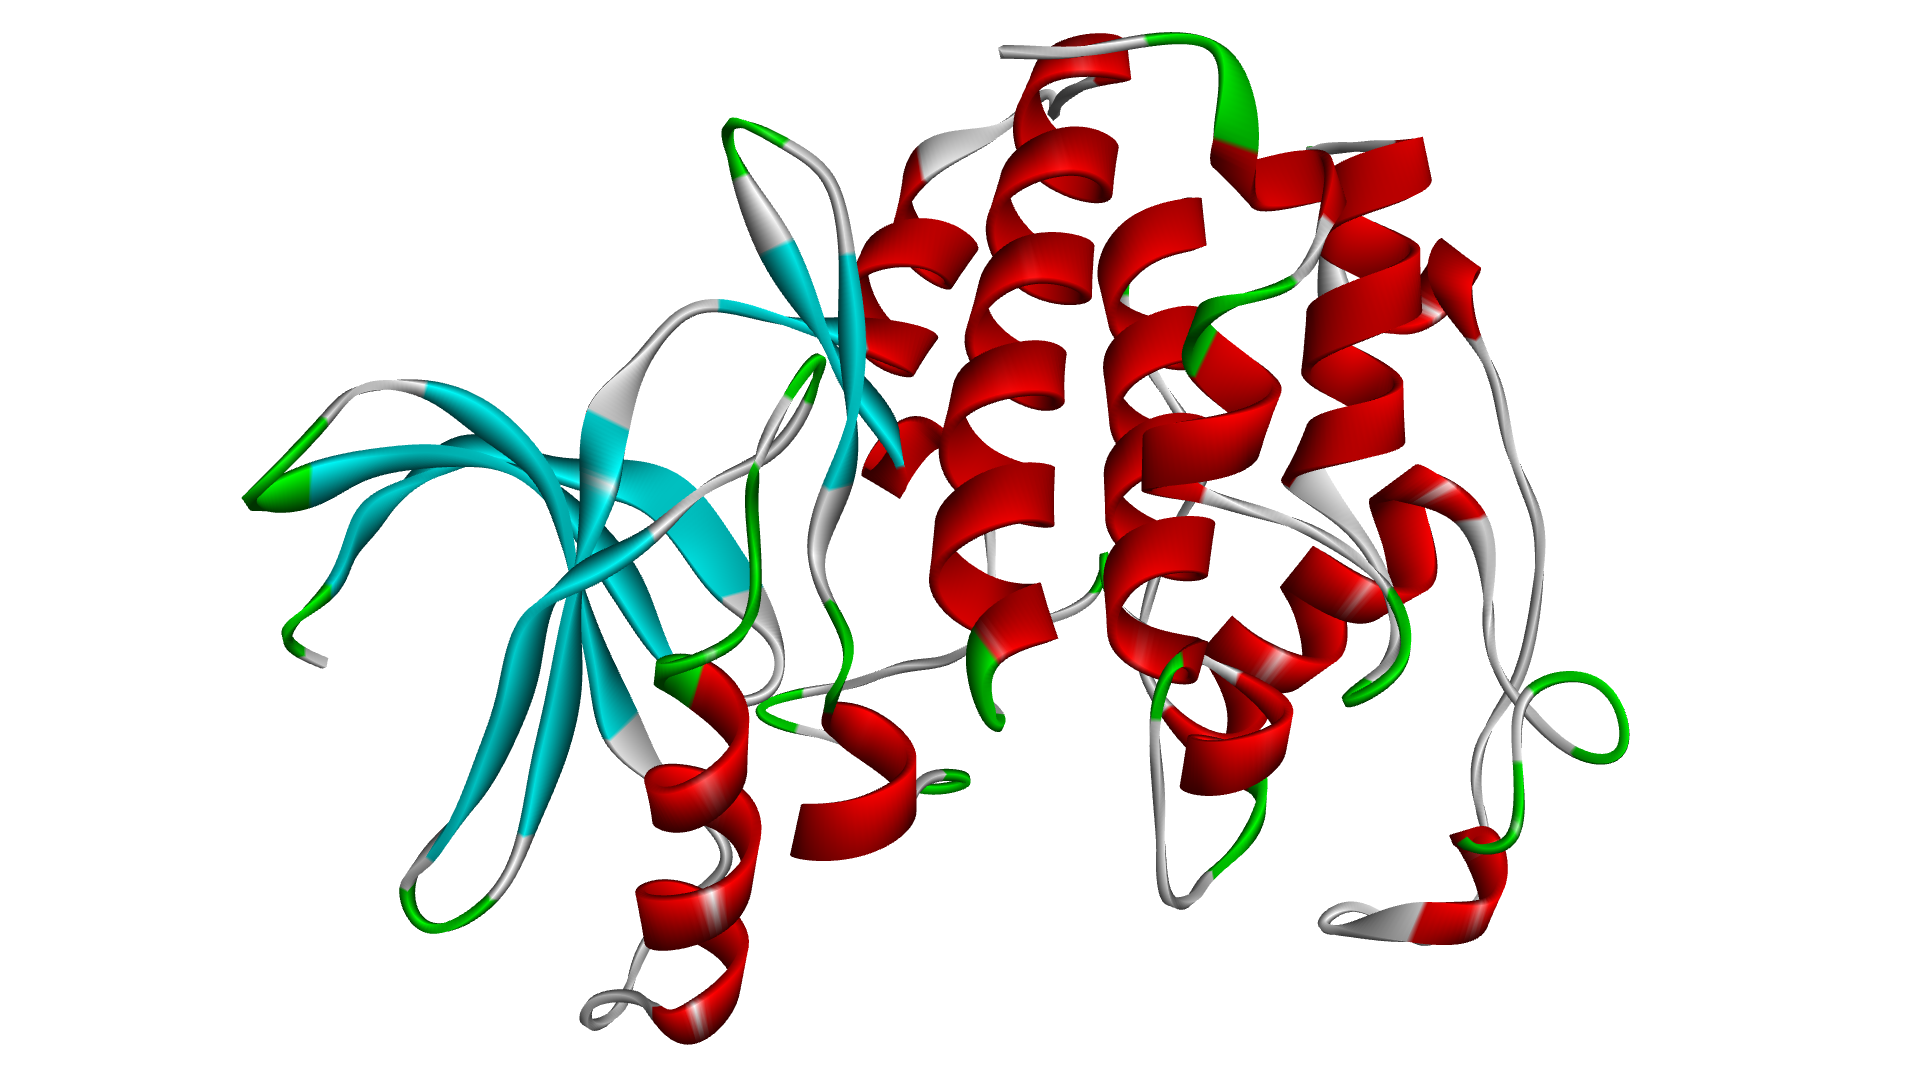
\includegraphics[width=\linewidth]{Case/CCRKHomologousModel.png}
\caption{CCRK homologous model, built on the CDK2 template with PDB ID 1HCL \citep{1142} using SWISS-MODEL.}
\label{Case:CCRKHomologousModel}
\end{figure}

\section{Cancer Stem Cells}

Prof. Hsiang-fu Kung and Dr. Hong Yao from Stanley Ho Centre for Emerging Infectious Diseases at Chinese University of Hong Kong are seeking specific therapies targeted at CSCs (Cancer Stem Cells) for improvement of survival and quality of life of cancer patients.

CSCs are cancer cells, found within tumors or hematological cancers, that possess the ability to give rise to all cell types found in a particular cancer sample. CSCs as the highly malignant seeds of tumors, typically comprising 1-5\% of the tumor, give rise to 95-99\% of other tumor cells known as the tumor bulk, and are therefore tumorigenic. While standard therapies, including chemotherapy and radiation, may initially shrink tumors by killing tumor bulk, the failure of these therapies to eradicate CSCs may be a major contributor to treatment failure, tumor relapse and poor survival (Figure \ref{Case:CancerStemCell}).

\begin{figure}
\centering
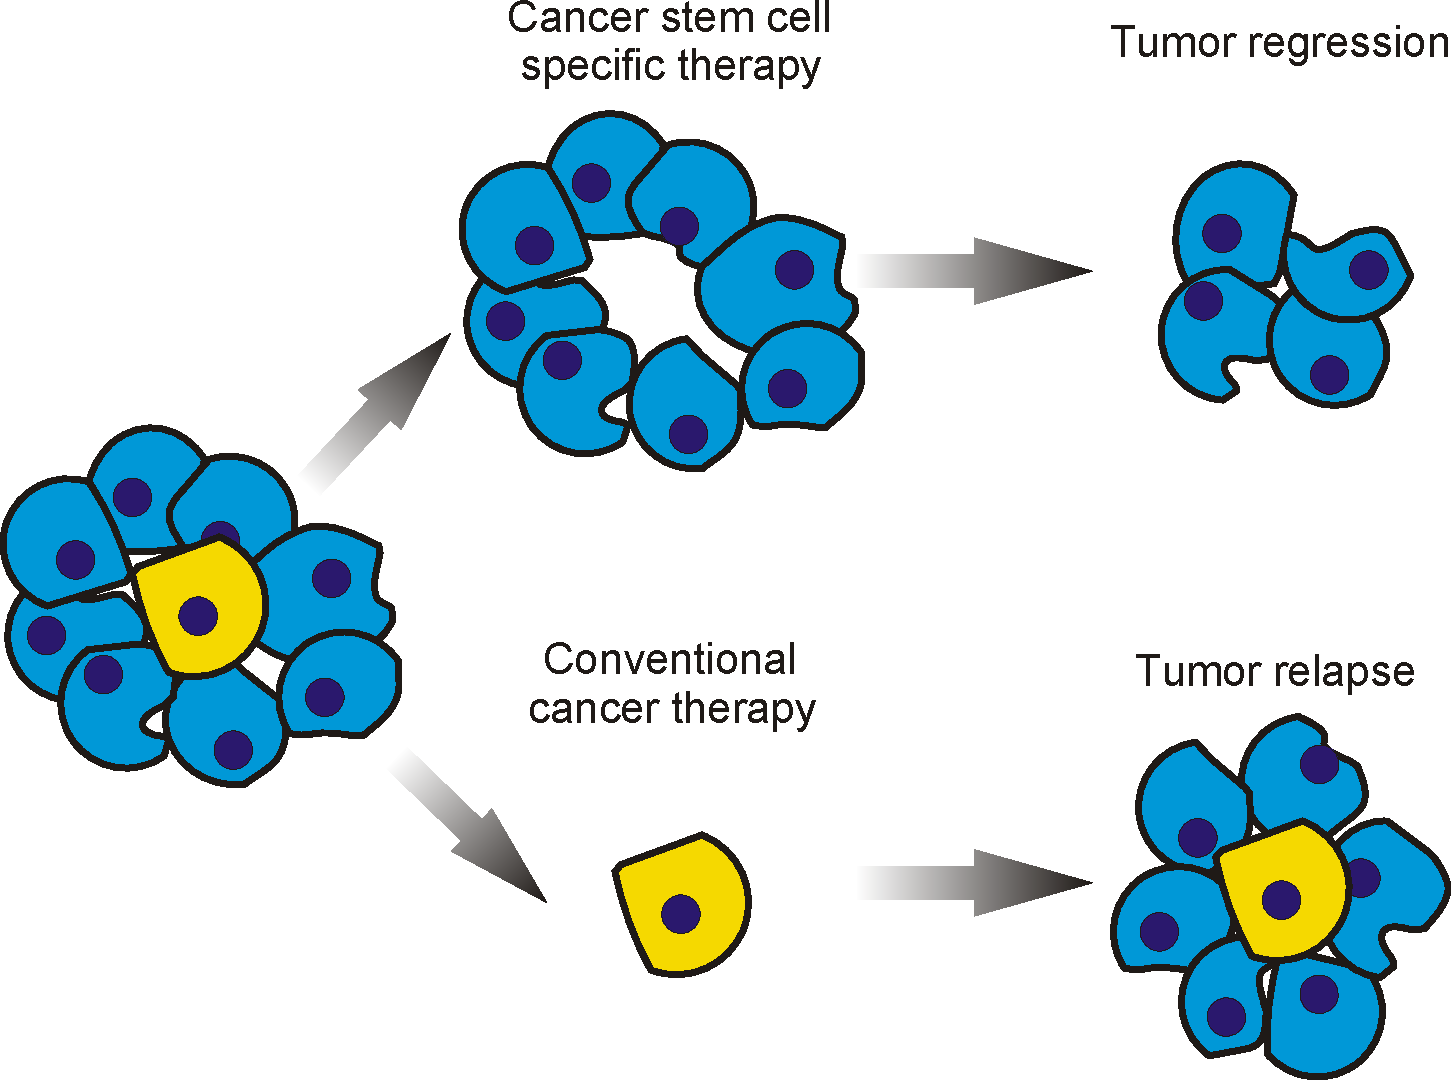
\includegraphics[width=\linewidth]{Case/CancerStemCell.pdf}
\caption{CSCs-specific and conventional cancer therapies. Cells in blue are normal cancer cells. Cells in yellow are CSCs. Source: Wikipedia.}
\label{Case:CancerStemCell}
\end{figure}

Salinomycin (Figure \ref{Case:SalinomycinEtoposideAbamectinNigericin}, reprinted from \citep{1147}), a monocarboxylic polyether antibiotic widely used as an anticoccidiosis agent in chicken, was discovered in a chemical screen to selectively kills breast CSCs and reduce the proportion of CSCs by >100-fold relative to paclitaxel, a commonly used breast cancer chemotherapeutic drug. Treatment of mice with salinomycin inhibits mammary tumor growth \textit{in vivo} and induces increased epithelial differentiation of tumor cells \citep{1147}. At the molecular mechanism level, salinomycin specifically inhibits the Wnt/$\beta$-catenin signaling pathway initiated by Wnt1 and selectively induces apoptosis in chronic lymphocytic leukemia cells \citep{1148}.

\begin{figure}
\centering
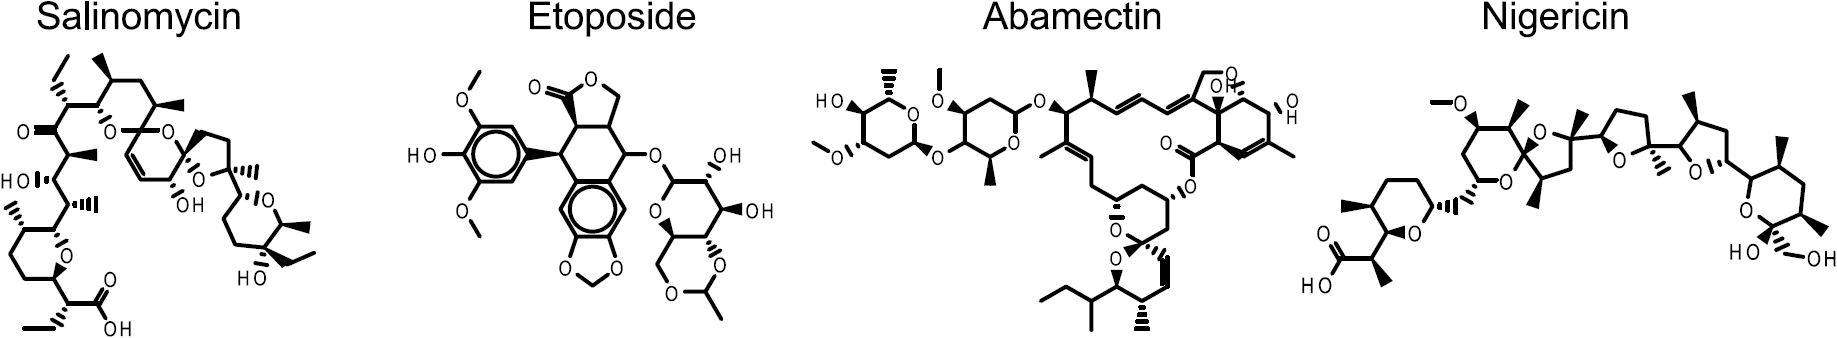
\includegraphics[width=\linewidth]{Case/SalinomycinEtoposideAbamectinNigericin.png}
\caption{Chemical structures of salinomycin, etoposide, abamectin, and nigericin, compounds that exhibit selective toxicity for mesenchymally transdifferentiated epithelial cells. Figure reprinted from \citep{1147}.}
\label{Case:SalinomycinEtoposideAbamectinNigericin}
\end{figure}

We confirm the Wnt protein as a potential pharmaceutical target of therapeutic interest. The major obstacle right now is the lack of resolved or homologous structures of Wnt. We can neither find a Wnt structure from the PDB database \citep{540,537}, nor predict its structure from known templates (Figure \ref{Case:WntHomologyModeling}). Although the 1JLT template shares 42\% sequence identity with Wnt, it only covers amino acids from 319 to 360. In contrast, the 1GTE template covers amino acids 13 to 354, but the sequence identity is as low as 14\%, far from sufficient for an accurate homologous model. In fact, we try five online homology modeling servers, namely ModWeb, M4T, SWISS-MODEL, I-TASSER, and HHpred, and most of them simply refuse our job just because of the surprisingly low sequence identity percentage. Therefore, one possible way to go is to explore another signaling pathways associated with CSCs, such as Bmi-1, Shh, Notch, \textit{Hox} family, Pten, etc.

\begin{figure}
\centering
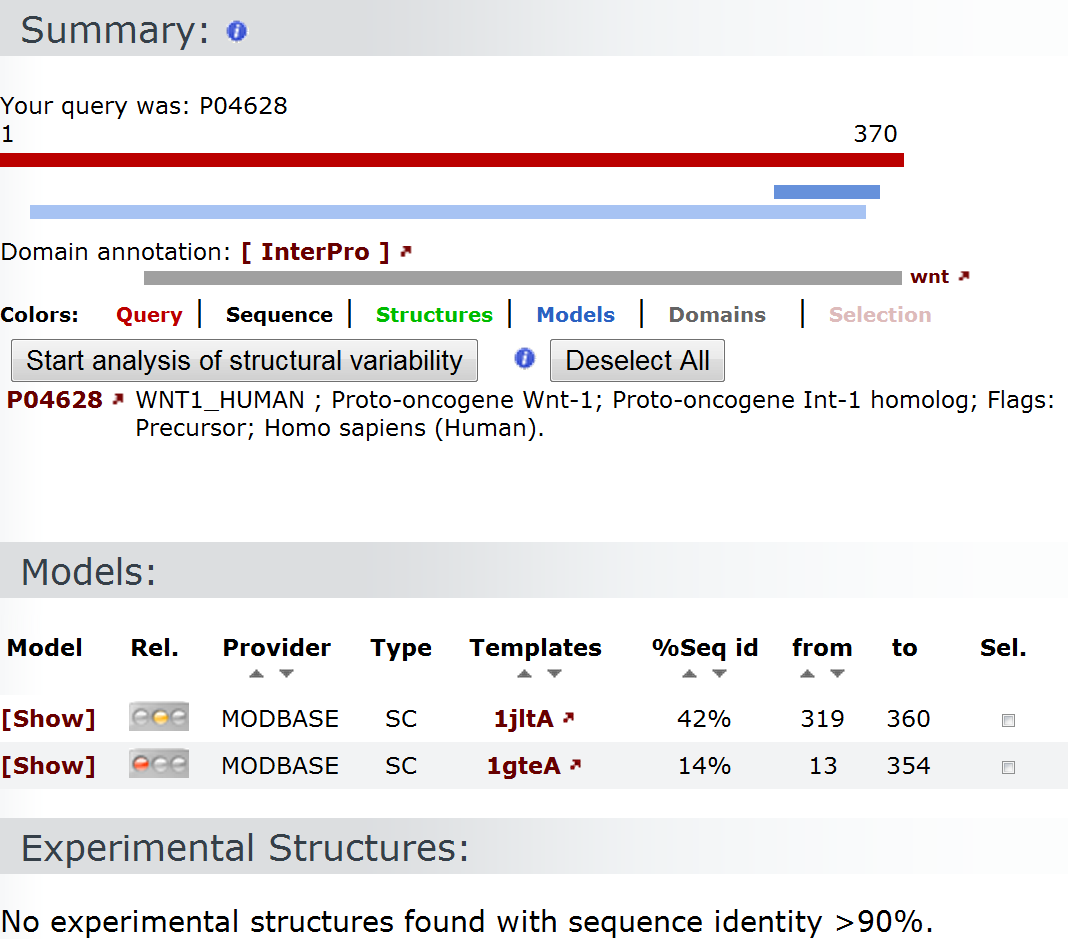
\includegraphics[width=\linewidth]{Case/WntHomologyModeling.png}
\caption{Proto-oncogene Wnt-1 of UniProt ID P04628 shares sequence identity with merely two templates, 1JLT chain A and 1GTE chain A. Source: The Protein Model Portal.}
\label{Case:WntHomologyModeling}
\end{figure}

\chapterend
